\setlength{\parindent}{2em} % 设置段落缩进为2em
\pagestyle{fancy}
\fancyhf{}
\fancyhead[C]{\leftmark}
\fancyfoot[C]{$\cdot$\thepage$\cdot$}
\renewcommand{\headrulewidth}{0.4pt}

\chapter{示例}
\section{示例}
\subsection{示例}

\begin{theorem}\label{exa}
	\begin{equation}\label{e1}
	Ax=b
 \end{equation}
\end{theorem}

\begin{definition}
	本模板使用的是cleveref,并且进行了自定义.例如可以引用\cref{exa} \cref{e1} \\
	这是引用公式的效果.
\end{definition}

\begin{method}
	本文也自定义了method环境.
\end{method}

\cite{1}本模板是按照被引用的前后顺序来给参考文献进行排序的\cite{2}.不过注意需要这样设置
\begin{figure}[h]
	\centering
	\begin{minipage}{0.65\linewidth}
		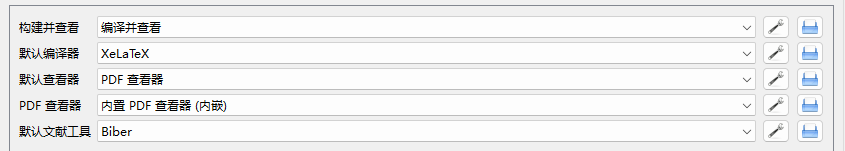
\includegraphics[width=\linewidth]{set.png}
		\caption{设置}
	\end{minipage}
\end{figure}
